\documentclass{article}
% Author: Luan Leal
% Last update: 2024-12-03

% ----------------------------

% ----------------------------   IMPORTS   ----------------------------
\usepackage{amssymb, amsthm, amsmath, geometry, siunitx, caption, float, graphicx}
\usepackage{enumitem}
\usepackage[utf8]{inputenc}
\usepackage[onehalfspacing]{setspaceenhanced}
\usepackage[brazil]{babel} % Adaptação ao pt-br
\usepackage{hyperref} % Usado para inserir links
\usepackage[capitalize, brazilian, noabbrev]{cleveref} % Referência adaptada ao pt-br
\usepackage{subcaption}
\usepackage{makecell}
\usepackage[num,overcite]{abntex2cite}

% ----------------------------   LAYOUT   ----------------------------
\citebrackets[]
\geometry{a4paper, lmargin=3cm, tmargin=3cm, rmargin=2cm, bmargin=2cm}
\onehalfspacing
%\setlength{\parindent}{45pt}
\sisetup{output-decimal-marker = {,}}

% ----------------------------  THEOREMS  ----------------------------
% -Ambiente de definição
\theoremstyle{definition}
\newtheorem{dfn}{Definição}[section]

% -Ambiente de observação
\theoremstyle{remark}
\newtheorem{obs}{Observação}

% -Ambiente de lema
\theoremstyle{definition}
\newtheorem{lema}{Lema}

% -Ambiente de exemplo
\theoremstyle{definition}
\newtheorem{xp}{Exemplo}[section]

% -Ambiente de proposição
\newtheorem{prop}{Proposição}

% -Ambiente de teorema e demonstração
\theoremstyle{plain}
\newtheorem{thm}{Teorema}
\theoremstyle{remark}
\newtheorem*{dms}{Demonstração}

% -Ambiente de exercício e resolução
\theoremstyle{definition}
\newtheorem{xcs}{Exercício}
\theoremstyle{remark}
\newtheorem*{rsl}{Resolução}

% ----------------------------  COMMANDS  ----------------------------
%\newcommand{\RR}{\mathbb{R}} % \mathbb{R} = \RR
%\newcommand{\ZZ}{\mathbb{Z}} % \mathbb{Z} = \ZZ

\author{Luan Leal (15470820); Matheus Justino (14598021); 
\\Matheus Queiroz (15479562); Micael Baruch (15578823)}
\title{Relatório 3} 

\captionsetup{margin=10pt,font=small,labelfont=bf,labelsep=period}

\begin{document}
\maketitle

\textbf{Questão 1}

\begin{figure}[H]
    \centering
    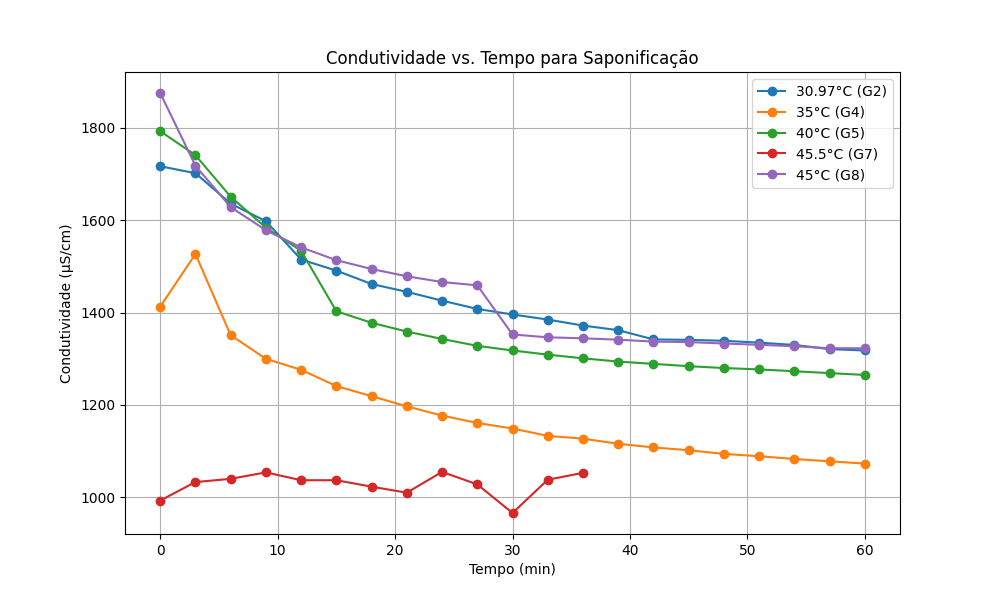
\includegraphics[width=.5\linewidth]{figs/graph1.png}
    \label{grafico1}
\end{figure}

\textbf{Questão 2}

\begin{figure}[H]
    \centering
    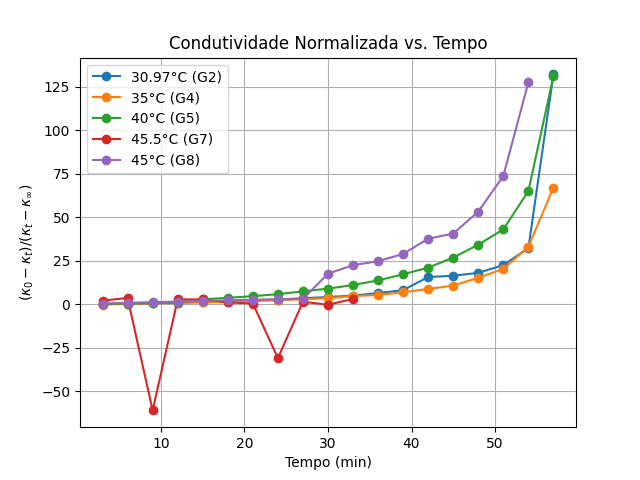
\includegraphics[width=.5\linewidth]{figs/graph2.png}
    \label{grafico2}
\end{figure}

De acordo com a equação \cref{EqdoGrafico} vemos que o gráfico deveria ter linhas retas que passam pela origem, e com inclinação igual a \(ak\). Porém, ao analisar o gráfico, observa-se que não houve o comportamento esperado, embora as curvas mostrem uma tendencia geral de crescimento, elas não são retas perfeitas, principalmente em tempos mais longos. Contudo, essa divergência é esperada, uma vez que os modelos cinéticos, como a equação \cref{EqdoGrafico}, funcionam melhor no inicio de reações, quando as concentrações de reagentes são altas e a influência da reação inversa e do acumulo de produtos ainda são mínimas. 
\begin{align}
	\frac{k_0 - k_t}{k_t - k_\infty} / t = ak
	\label{EqdoGrafico}
\end{align}
\textbf{Questão 3}

\begin{figure}[H]
    \centering
    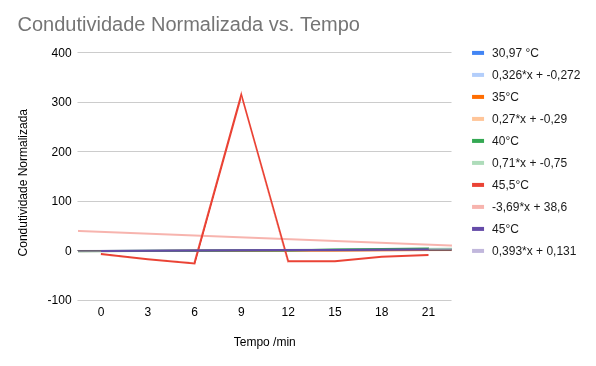
\includegraphics[width=.5\linewidth]{figs/graph3.png}
    \label{grafico3}
\end{figure}
Como a regressão linear do experimento a 45$^{\circ}$C resultou em um coeficiente angular negativo, o que é impossível para a reação que estamos analisando, optou-se por omitir seus dados para futuros cálculos mais precisos.
\begin{figure}[H]
	\centering
	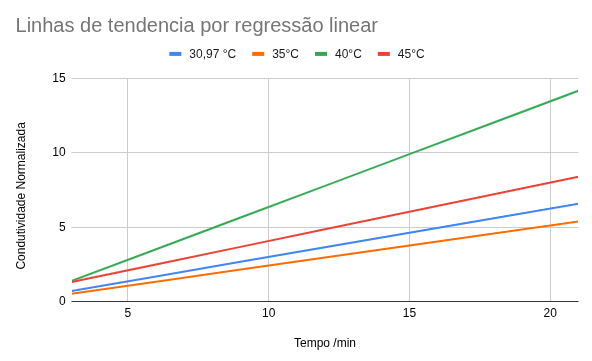
\includegraphics[width=.5\linewidth]{figs/LinhaTendencia.png}
	\label{grafico4}
\end{figure}
O comportamento linear do início da reação ocorre pois no início as concentrações dos reagentes são altas e a influência da reação inversa ou de produtos é mínima. Nessas condições ideais, a reação segue o modelo cinético de forma mais previsível, resultando em um comportamento linear no gráfico.

\textbf{Questão 4}

A partir da equação \cref{EqdoGrafico}, observamos que o gráfico de Linhas de tendencia por regressão linear, é descrito por ela. Então ao analisar a equação, vê-se que, como descreve uma equação de reta, o coeficiente angular de cada reta seria igual a \(ak\).
Dessa forma, podemos calcular o valor de \(k\) para cada temperatura usando a equação \cref{konstante}. Sabendo que \(a = \frac{0,0197 mol/L}{2} = 0,00985 mol/L\) 
\begin{align}
	\frac{\text{(inclinação)}}{a} = k
	\label{konstante}
\end{align}

\begin{table}[H]
\centering
\caption{Valores de $k$ em diferentes temperaturas.}
\label{tab:k_norm}
\begin{tabular}{lrrrrrrr}
\toprule
\textbf{Temperatura ($^{\circ}$C)}    & \textbf{inclinação ($ak$)} & {\textbf{k}} \\
\midrule
30.97 (G2) & 0,326 & 33,1\\
35 (G4)    & 0,27 & 27,41\\
40 (G5)    & 0,71 & 72,08\\
45 (G8)    & 0,393 & 39,89\\
\bottomrule
\end{tabular}
\end{table}
\textbf{Questão 5}

 Dada  equação \cref{Energiadeativação}, podemos analisa-la como uma equação de reta, da forma \(y = mx + b\), em que \( y = ln (k)\) , \(x = \frac{1}{T}  \) e \( m = -\frac{E_a}{R}\), possibilitando a construção do gráfico de Arrhenius para a reação de saponificação.
 \begin{align}
	ln(k) = (-\frac{E_a}{R}) \frac{1}{T} + ln(A)
	\label{Energiadeativação}
 \end{align}
A partir das informações obtidas foi possível construir o gráfico de Arrhenius, e assim, ao construir uma linha de tendência por regressão linear, obteve-se uma equação de reta \(y = 3189*x + 14\). 
\begin{figure}[H]
	\centering
	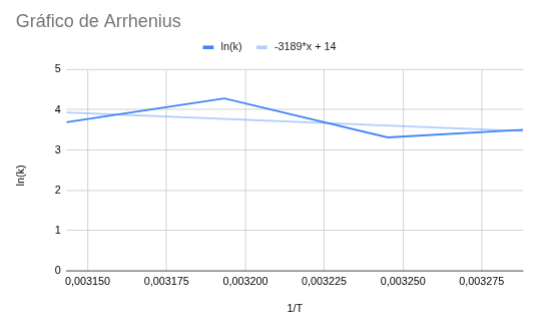
\includegraphics[width=.5\linewidth]{figs/Arrhenius.png}
	\label{Arrhenius}
\end{figure}
E como foi descrito anteriormente, sabemos que \( m = -\frac{E_a}{R}\) e como descrito pela equação de reta do gráfico de Arrhenius, temos um \(m = -3189\). Dessa forma, assumindo um \(R = 8,314 J/mol*K\), temos que a Energia de Ativação será: 
\begin{align*}
	3189 = \frac{E_a}{8,314 } = 26513,346 J = 26,51 kJ
\end{align*}


\textbf{Questão 6}

Não é correto utilizar a primeira medida após a mistura dos reagentes como valor de tempo zero, pois a reação de saponificação começa imediatamente após o hidróxido de sódio \(NaOH\) e o acetato de etila entrarem em contato. Por isso deve-se utilizar a solução de puro Hidróxido de sódio, descrita no passo 7, porque ela representa a condutividade inicial, antes de começar a ocorrer a reação efetivamente. 


\textbf{Questão 7}

Desconsiderando erros no preparo das soluções, a maior fonte de erro neste experimento é a flutuação da temperatura.
A determinação da constante de velocidade (\(k\)) e, principalmente, da energia de ativação (\(E_a\)), é extremamente sensível à temperatura. A relação entre a constante de velocidade e a temperatura é descrita pela equação de Arrhenius, mostrando que essa dependência é exponencial, o que significa que mesmo uma pequena variação na temperatura pode causar uma mudança significativa no valor da constante de velocidade.
Qualquer falha em manter a temperatura rigorosamente constante afetará a velocidade da reação ao longo do tempo, levando a um valor de \(k\) incorreto para aquela temperatura. Como o cálculo da Energia de Ativação depende da comparação de valores de \(k\) obtidos em diferentes temperaturas, um erro no controle da temperatura em qualquer um dos ensaios comprometerá diretamente o resultado final da Energia de ativação.

  
\end{document}
